% ============================================================
% content/questions.tex —— 2018 全国Ⅰ卷（理综物理部分）· 试题
% 来源：中国教育在线公开原卷 Word 版（原卷 docx，含官方答案与解析）
% 题号保留官方编号 14--21、22--25、33--34；第 1--13 题为理综其他科目。
% 图形见 figures/（全部为 TikZ/circuitikz/pgfplots 矢量重绘）
% ============================================================

\begin{gknotice}
  \textbf{卷种说明：}本卷为 2018 年普通高等学校招生全国统一考试理科综合能力测试（全国卷Ⅰ）的物理部分，
  满分 110 分，考试用时 90 分钟。选择题题号从 14 开始，因为第 1--13 题为理综其他科目试题，
  本工程只收录物理部分。第 33、34 题为选考题（选修 3-3、选修 3-4），考生按原卷要求任选一题作答。
\end{gknotice}

\gkpart{二、选择题}

\textbf{（本题共 8 小题，每小题 6 分，共 48 分。在每小题给出的四个选项中，第 14--18 题只有一项符合题目要求，第 19--21 题有多项符合题目要求。全部选对的得 6 分，选对但不全的得 3 分，有选错的得 0 分。）}

\begin{question}
\gkti{14}高铁列车在启动阶段的运动可看作初速度为零的匀加速直线运动，在启动阶段列车的动能\gkblank

\begin{gkopts}(1)
  \task A．与它所经历的时间成正比
  \task B．与它的位移成正比
  \task C．与它的速度成正比
  \task D．与它的动量成正比
\end{gkopts}
\end{question}

\begin{question}
\gkti{15}如图，轻弹簧的下端固定在水平桌面上，上端放有物块 $P$，系统处于静止状态。现用一竖直向上的力 $F$ 作用在 $P$ 上，使其向上做匀加速直线运动。以 $x$ 表示 $P$ 离开静止位置的位移，在弹簧恢复原长前，下列表示 $F$ 和 $x$ 之间关系的图像可能正确的是\gkblank

\gkfig{figures/q15-setup}

\begin{gkopts}(4)
  \task A．% 第 15 题选项 A：F–x 图为过纵轴正截距的上升直线
\begin{tikzpicture}[font=\scriptsize, scale=0.62]
  \draw[->] (0,0) -- (2.5,0) node[right] {$x$};
  \draw[->] (0,0) -- (0,2.2) node[above] {$F$};
  \node[below left] at (0,0) {$O$};
  \draw[thick] (0,0.55) -- (2.1,1.9);
\end{tikzpicture}

  \task B．% 第 15 题选项 B：F–x 图为过原点的上升直线
\begin{tikzpicture}[font=\scriptsize, scale=0.62]
  \draw[->] (0,0) -- (2.5,0) node[right] {$x$};
  \draw[->] (0,0) -- (0,2.2) node[above] {$F$};
  \node[below left] at (0,0) {$O$};
  \draw[thick] (0,0) -- (2.1,1.9);
\end{tikzpicture}

  \task C．% 第 15 题选项 C：F 不随 x 变化的水平线
\begin{tikzpicture}[font=\scriptsize, scale=0.62]
  \draw[->] (0,0) -- (2.5,0) node[right] {$x$};
  \draw[->] (0,0) -- (0,2.2) node[above] {$F$};
  \node[below left] at (0,0) {$O$};
  \draw[thick] (0,1.3) -- (2.0,1.3);
\end{tikzpicture}

  \task D．% 第 15 题选项 D：F–x 先过原点线性上升、后跳变再线性上升的折线
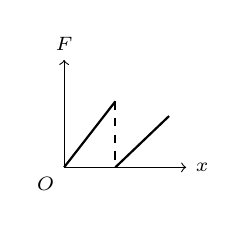
\begin{tikzpicture}[font=\scriptsize, scale=0.62]
  \draw[->] (0,0) -- (2.5,0) node[right] {$x$};
  \draw[->] (0,0) -- (0,2.2) node[above] {$F$};
  \node[below left] at (0,0) {$O$};
  \draw[thick] (0,0) -- (1.05,1.35);
  \draw[thick,dashed] (1.05,1.35) -- (1.05,0);
  \draw[thick] (1.05,0) -- (2.15,1.05);
\end{tikzpicture}

\end{gkopts}
\end{question}

\begin{question}
\gkti{16}如图，三个固定的带电小球 $a$、$b$ 和 $c$，相互间的距离分别为 $ab=\SI{5}{\centi\metre}$，$bc=\SI{3}{\centi\metre}$，$ca=\SI{4}{\centi\metre}$。小球 $c$ 所受库仑力的合力的方向平行于 $a$、$b$ 的连线。设小球 $a$、$b$ 所带电荷量的比值的绝对值为 $k$，则\gkblank

\gkfig{figures/q16-balls}

\begin{gkopts}(2)
  \task A．$a$、$b$ 的电荷同号，$k=\dfrac{16}{9}$
  \task B．$a$、$b$ 的电荷异号，$k=\dfrac{16}{9}$
  \task C．$a$、$b$ 的电荷同号，$k=\dfrac{64}{27}$
  \task D．$a$、$b$ 的电荷异号，$k=\dfrac{64}{27}$
\end{gkopts}
\end{question}

\begin{question}
\gkti{17}如图，导体轨道 $OPQS$ 固定，其中 $PQS$ 是半圆弧，$Q$ 为半圆弧的中点，$O$ 为圆心，轨道的电阻忽略不计。$OM$ 是有一定电阻、可绕 $O$ 转动的金属杆，$M$ 端位于 $PQS$ 上，$OM$ 与轨道接触良好。空间存在与半圆所在平面垂直的匀强磁场，磁感应强度的大小为 $B$。现使 $OM$ 从 $OQ$ 位置以恒定的角速度逆时针转到 $OS$ 位置并固定（过程Ⅰ）；再使磁感应强度的大小以一定的变化率从 $B$ 增加到 $B'$（过程Ⅱ）。在过程Ⅰ、Ⅱ中，流过 $OM$ 的电荷量相等，则 $\dfrac{B'}{B}$ 等于\gkblank

\gkfig{figures/q17-frame}

\begin{gkopts}(4)
  \task A．$\dfrac{5}{4}$
  \task B．$\dfrac{3}{2}$
  \task C．$\dfrac{7}{4}$
  \task D．$2$
\end{gkopts}
\end{question}

\begin{question}
\gkti{18}如图，$abc$ 是竖直面内的光滑固定轨道，$ab$ 水平，长度为 $2R$；$bc$ 是半径为 $R$ 的四分之一圆弧，与 $ab$ 相切于 $b$ 点。一质量为 $m$ 的小球，始终受到与重力大小相等的水平外力的作用，自 $a$ 点处从静止开始向右运动。重力加速度大小为 $g$。小球从 $a$ 点开始运动到其轨迹最高点，机械能的增量为\gkblank

\gkfig{figures/q18-track}

\begin{gkopts}(4)
  \task A．$2mgR$
  \task B．$4mgR$
  \task C．$5mgR$
  \task D．$6mgR$
\end{gkopts}
\end{question}

\begin{question}
\gkti{19}如图，两个线圈绕在同一根铁芯上，其中一线圈通过开关与电源连接，另一线圈与远处沿南北方向水平放置在纸面内的直导线连接成回路。将一小磁针悬挂在直导线正上方，开关未闭合时小磁针处于静止状态。下列说法正确的是\gkblank

\gkfig{figures/q19-coils}

\begin{gkopts}(1)
  \task A．开关闭合后的瞬间，小磁针的 N 极朝垂直纸面向里的方向转动
  \task B．开关闭合并保持一段时间后，小磁针的 N 极指向垂直纸面向里的方向
  \task C．开关闭合并保持一段时间后，小磁针的 N 极指向垂直纸面向外的方向
  \task D．开关闭合并保持一段时间再断开后的瞬间，小磁针的 N 极朝垂直纸面向外的方向转动
\end{gkopts}
\end{question}

\begin{question}
\gkti{20}2017 年，人类第一次直接探测到来自双中子星合并的引力波。根据科学家们复原的过程，在两颗中子星合并前约 \SI{100}{\second} 时，它们相距约 \SI{400}{\kilo\metre}，绕二者连线上的某点每秒转动 12 圈。将两颗中子星都看作是质量均匀分布的球体，由这些数据、万有引力常量并利用牛顿力学知识，可以估算出这一时刻两颗中子星\gkblank

\begin{gkopts}(1)
  \task A．质量之积
  \task B．质量之和
  \task C．速率之和
  \task D．各自的自转角速度
\end{gkopts}
\end{question}

\begin{question}
\gkti{21}图中虚线 $a$、$b$、$c$、$d$、$f$ 代表匀强电场内间距相等的一组等势面，已知平面 $b$ 上的电势为 \SI{2}{\volt}。一电子经过 $a$ 时的动能为 \SI{10}{eV}，从 $a$ 到 $d$ 的过程中克服电场力所做的功为 \SI{6}{eV}。下列说法正确的是\gkblank

\gkfig{figures/q21-surfaces}

\begin{gkopts}(1)
  \task A．平面 $c$ 上的电势为零
  \task B．该电子可能到达不了平面 $f$
  \task C．该电子经过平面 $d$ 时，其电势能为 \SI{4}{eV}
  \task D．该电子经过平面 $b$ 时的速率是经过 $d$ 时的 2 倍
\end{gkopts}
\end{question}

\gkpart{三、非选择题}

\textbf{（共 62 分。第 22--25 题为必考题，每个试题考生都必须作答。第 33--34 题为选考题，考生根据要求作答。）}

\gksubpart{（一）必考题（共 47 分）}

\begin{question}
\gkti{22}（5 分）如图（a），一弹簧上端固定在支架顶端，下端悬挂一托盘；一标尺由游标和主尺构成，主尺竖直固定在弹簧左边；托盘上方固定有一能与游标刻度线准确对齐的装置，简化为图中的指针。

现要测量图（a）中弹簧的劲度系数。当托盘内没有砝码时，移动游标，使其零刻度线对准指针，此时标尺读数为 \SI{1.950}{\centi\metre}；当托盘内放有质量为 \SI{0.100}{\kilogram} 的砝码时，移动游标，再次使其零刻度线对准指针，标尺示数如图（b）所示，其读数为\gkblank \si{\centi\metre}。当地的重力加速度大小为 \SI{9.80}{\metre\per\second\squared}，此弹簧的劲度系数为\gkblank \si{\newton\per\metre}（保留 3 位有效数字）。

\gkfig{figures/q22-vernier}
\end{question}

\begin{question}
\gkti{23}（10 分）某实验小组利用如图（a）所示的电路探究在 $25\,^{\circ}\mathrm{C}$--$80\,^{\circ}\mathrm{C}$ 范围内某热敏电阻的温度特性。所用器材有：置于温控室（图中虚线区域）中的热敏电阻 $R_{T}$，其标称值（$25\,^{\circ}\mathrm{C}$ 时的阻值）为 \SI{900.0}{\ohm}；电源 $E$（\SI{6}{\volt}，内阻可忽略）；电压表（量程 \SI{150}{\milli\volt}）；定值电阻 $R_{0}$（阻值 \SI{20.0}{\ohm}）；滑动变阻器 $R_{1}$（最大阻值为 \SI{1000}{\ohm}）；电阻箱 $R_{2}$（阻值范围 $0$--\SI{999.9}{\ohm}）；单刀开关 $\mathrm{S}_{1}$，单刀双掷开关 $\mathrm{S}_{2}$。

\gkfig{figures/q23-circuit}

实验时，先按图（a）连接好电路，再将温控室的温度 $t$ 升至 $80.0\,^{\circ}\mathrm{C}$，将 $\mathrm{S}_{2}$ 与 1 端接通，闭合 $\mathrm{S}_{1}$，调节 $R_{1}$ 的滑片位置，使电压表读数为某一值 $U_{0}$；保持 $R_{1}$ 的滑片位置不变，将 $R_{2}$ 置于最大值，将 $\mathrm{S}_{2}$ 与 2 端接通，调节 $R_{2}$，使电压表读数仍为 $U_{0}$；断开 $\mathrm{S}_{1}$，记下此时 $R_{2}$ 的读数。逐步降低温控室的温度 $t$，得到相应温度下 $R_{2}$ 的阻值，直至温度降到 $25.0\,^{\circ}\mathrm{C}$。实验得到的 $R_{2}$--$t$ 数据见下表。

\begin{center}
\small
\begin{tabular}{@{}lccccccc@{}}
\toprule
$t/\,^{\circ}\mathrm{C}$ & 25.0 & 30.0 & 40.0 & 50.0 & 60.0 & 70.0 & 80.0\\
\midrule
$R_{2}/\si{\ohm}$ & 900.0 & 680.0 & 500.0 & 390.0 & 320.0 & 270.0 & 240.0\\
\bottomrule
\end{tabular}
\end{center}

回答下列问题：
\begin{enumerate}[leftmargin=2em, label=(\arabic*)]
  \item 在闭合 $\mathrm{S}_{1}$ 前，图（a）中 $R_{1}$ 的滑片应移动到\gkblank（填“$a$”或“$b$”）端。
  \item 在图（b）的坐标纸上补齐数据表中所给数据点，并作出 $R_{2}$--$t$ 曲线。
  \item 由图（b）可得到 $R_{T}$ 在 $25\,^{\circ}\mathrm{C}$--$80\,^{\circ}\mathrm{C}$ 范围内的温度特性。当 $t=44.0\,^{\circ}\mathrm{C}$ 时，可得 $R_{T}=$\gkblank $\Omega$。
  \item 将 $R_{T}$ 握于手心，手心温度下 $R_{2}$ 的相应读数如图（c）所示，该读数为\gkblank $\Omega$，则手心温度为\gkblank $\,^{\circ}\mathrm{C}$。
\end{enumerate}

\gkfig{figures/q23-grid}

\gkfig{figures/q23-dial}
\end{question}

\begin{question}
\gkti{24}（12 分）一质量为 $m$ 的烟花弹获得动能 $E$ 后，从地面竖直升空。当烟花弹上升的速度为零时，弹中火药爆炸将烟花弹炸为质量相等的两部分，两部分获得的动能之和也为 $E$，且均沿竖直方向运动。爆炸时间极短，重力加速度大小为 $g$，不计空气阻力和火药的质量。求：
\begin{enumerate}[leftmargin=2em, label=(\arabic*)]
  \item 烟花弹从地面开始上升到弹中火药爆炸所经过的时间；
  \item 爆炸后烟花弹向上运动的部分距地面的最大高度。
\end{enumerate}
\end{question}

\begin{question}
\gkti{25}（20 分）如图，在 $y>0$ 的区域存在方向沿 $y$ 轴负方向的匀强电场，场强大小为 $E$；在 $y<0$ 的区域存在方向垂直于 $xOy$ 平面向外的匀强磁场。一个氕核 ${}_{1}^{1}\mathrm{H}$ 和一个氘核 ${}_{1}^{2}\mathrm{H}$ 先后从 $y$ 轴上 $y=h$ 点以相同的动能射出，速度方向沿 $x$ 轴正方向。已知 ${}_{1}^{1}\mathrm{H}$ 进入磁场时，速度方向与 $x$ 轴正方向的夹角为 $60^{\circ}$，并从坐标原点 $O$ 处第一次射出磁场。${}_{1}^{1}\mathrm{H}$ 的质量为 $m$，电荷量为 $q$，不计重力。求：
\begin{enumerate}[leftmargin=2em, label=(\arabic*)]
  \item ${}_{1}^{1}\mathrm{H}$ 第一次进入磁场的位置到原点 $O$ 的距离；
  \item 磁场的磁感应强度大小；
  \item ${}_{1}^{2}\mathrm{H}$ 第一次离开磁场的位置到原点 $O$ 的距离。
\end{enumerate}

\gkfig{figures/q25-region}
\end{question}

\gksubpart{（二）选考题（共 15 分。请考生从 2 道物理题中任选一题作答。如果多做，则按所做的第一题计分。）}

\begin{question}
\gkti{33}[物理——选修 3-3]

(1)（5 分）如图，一定质量的理想气体从状态 $a$ 开始，经历过程①、②、③、④到达状态 $e$。对此气体，下列说法正确的是\gkblank（选对 1 个得 2 分，选对 2 个得 4 分，选对 3 个得 5 分；每选错 1 个扣 3 分，最低得分为 0 分）

\gkfig{figures/q33-cycle}

\begin{gkopts}(1)
  \task A．过程①中气体的压强逐渐减小
  \task B．过程②中气体对外界做正功
  \task C．过程④中气体从外界吸收了热量
  \task D．状态 $c$、$d$ 的内能相等
  \task E．状态 $d$ 的压强比状态 $b$ 的压强小
\end{gkopts}

(2)（10 分）如图，容积为 $V$ 的汽缸由导热材料制成，面积为 $S$ 的活塞将汽缸分成容积相等的上下两部分，汽缸上部通过细管与装有某种液体的容器相连，细管上有一阀门 $K$。开始时，$K$ 关闭，汽缸内上下两部分气体的压强均为 $p_{0}$。现将 $K$ 打开，容器内的液体缓慢地流入汽缸，当流入的液体体积为 $\dfrac{V}{8}$ 时，将 $K$ 关闭，活塞平衡时其下方气体的体积减小了 $\dfrac{V}{6}$。不计活塞的质量和体积，外界温度保持不变，重力加速度大小为 $g$。求流入汽缸内液体的质量。

\gkfig{figures/q33-cylinder}
\end{question}

\begin{question}
\gkti{34}[物理——选修 3-4]

(1)（5 分）如图，$\triangle ABC$ 为一玻璃三棱镜的横截面，$\angle A=30^{\circ}$。一束红光垂直 $AB$ 边射入，从 $AC$ 边上的 $D$ 点射出，其折射角为 $60^{\circ}$，则玻璃对红光的折射率为\gkblank。若改用蓝光沿同一路径入射，则光线在 $D$ 点射出时的折射角\gkblank（填“小于”“等于”或“大于”）$60^{\circ}$。

\gkfig{figures/q34-prism}

(2)（10 分）一列简谐横波在 $t=\dfrac{1}{3}\,\si{\second}$ 时的波形图如图（a）所示，$P$、$Q$ 是介质中的两个质点，图（b）是质点 $Q$ 的振动图像。求：
\begin{enumerate}[leftmargin=2em, label=(\roman*)]
  \item 波速及波的传播方向；
  \item 质点 $Q$ 的平衡位置的 $x$ 坐标。
\end{enumerate}

\gkfig{figures/q34-wave}
\end{question}
